%%%%%%%%%%%%%%%%%%%%%%%%%%%%%%%%%%%%%%%%%%%%%%%%%%%%%%%%%%%%%%%%%%%%%%
%% language specification:
%%   Here you define in which langugage your paper will be written.
%%   There are ALWAYS 2 languages to define (even you do not need it.)
%%   Since we are writing only in German or English, other languages
%%   are not supported.
%%   Choose either 'german' or 'english' as your first language.
\newcommand{\myfirstlang}{english}
%%%%%%%%%%%%%%%%%%%%%%%%%%%%%%%%%%%%%%%%%%%%%%%%%%%%%%%%%%%%%%%%%%%%%%

%%%%%%%%%%%%%%%%%%%%%%%%%%%%%%%%%%%%%%%%%%%%%%%%%%%%%%%%%%%%%%%%%%%%%%
%% Include Paper-Layout:
%%   Here the journal layout is chosen:
%%   Just now, only two possibilities are supported
%%   journal=workpaper  - the ivt internal workpaper layout  
%%   jornal=trb         - the so called trb layout 
%% !TeX encoding = usascii
% Prepare to get rid of \mypath one day
\providecommand\mypath[3]{}
%%%%%%%%%%%%%%%%%%%%%%%%%%%%%%%%%%%%%%%%%%%%%%%%%%%%%%%%%%%%%%%%%%%%%%
%% $Id$
%%%%%%%%%%%%%%%%%%%%%%%%%%%%%%%%%%%%%%%%%%%%%%%%%%%%%%%%%%%%%%%%%%%%%%

%%%%%%%%%%%%%%%%%%%%%%%%%%%%%%%%%%%%%%%%%%%%%%%%%%%%%%%%%%%%%%%%%%%%%%
%%
%% IVT WORKING PAPER LAYOUT (BASED ON IVT GENERIC LAYOUT)
%% Date: 2010-08-06
%% author:
%%   Kirill M\"uller, muelleki@ethz.ch
%%
%%%%%%%%%%%%%%%%%%%%%%%%%%%%%%%%%%%%%%%%%%%%%%%%%%%%%%%%%%%%%%%%%%%%%%

\newcommand{\internpapertype}{%
  \iflanguage{english}{Working paper}{%
    \iflanguage{german}{Arbeitsberichte}{%
      \langerrmessage}}}
\newcommand{\myinternpapertypeandnumber}{%
  \large\textbf{\internpapertype} & \large\textbf{\mynumber} \\[1ex]
}
\newcommand{\myinterninstitutionforabstract}{
  \internpapertype\iflanguage{german}{\ \interninstitution}{} & \mynumber \\
}
\newcommand{\interncitation}{%
  \internauthorstring%
  (\myyear) \mytitle, \emph{\internpapertype\iflanguage{german}{\ \interninstitution}{}}, \textbf{\mynumber}, %
  \iflanguage{english}{%
    Institute for Transport Planning and Systems (IVT), ETH Zurich, Zurich.%
  }{%
    \iflanguage{german}{%
      Institut f\"ur Verkehrsplanung und Transportsysteme (IVT), ETH Z\"urich, Z\"urich.%
    }{%
      \langerrmessage%
    }%
  }%
}
% !TeX encoding = usascii
% Prepare to get rid of \mypath one day
\providecommand\mypath[3]{}
%%%%%%%%%%%%%%%%%%%%%%%%%%%%%%%%%%%%%%%%%%%%%%%%%%%%%%%%%%%%%%%%%%%%%%
%% $Id$
%%%%%%%%%%%%%%%%%%%%%%%%%%%%%%%%%%%%%%%%%%%%%%%%%%%%%%%%%%%%%%%%%%%%%%

%%%%%%%%%%%%%%%%%%%%%%%%%%%%%%%%%%%%%%%%%%%%%%%%%%%%%%%%%%%%%%%%%%%%%%
%%
%% IVT GENERIC PAPER LAYOUT FOR KOMA SCRIPT
%% Date: 2010-04-05
%% author:
%%   Kirill M\"uller, muelleki@ivt.baug.ethz.ch
%%
%%%%%%%%%%%%%%%%%%%%%%%%%%%%%%%%%%%%%%%%%%%%%%%%%%%%%%%%%%%%%%%%%%%%%%

%%%%%%%%%%%%%%%%%%%%%%%%%%%%%%%%%%%%%%%%%%%%%%%%%%%%%%%%%%%%%%%%%%%%%%
%%%%%%%%%%%%%%%%%%%%%%%%%%%%%%%%%%%%%%%%%%%%%%%%%%%%%%%%%%%%%%%%%%%%%%
%%
%% Standard latex layout configurations
%%   Here, commands and settings are use which are available
%%   by the latex packages
%%
%%%%%%%%%%%%%%%%%%%%%%%%%%%%%%%%%%%%%%%%%%%%%%%%%%%%%%%%%%%%%%%%%%%%%%
%%%%%%%%%%%%%%%%%%%%%%%%%%%%%%%%%%%%%%%%%%%%%%%%%%%%%%%%%%%%%%%%%%%%%%
%% Type of document:
%% - Paperformat: letterpaper, a4paper, a5paper, b5paper,
%%   executivepaper, legalpaper
%% - Main font size: 10pt, 11pt, 12pt
%% - Formulae setting: - (centred), fleqn (left-aligned)
%% - Numbering of formulae: - (right-aligned), leqno (left-aligned)
%% - New page after title: titlepage, notitlepage
%% - Number of columns per page: onecolumn, twocolumn
%% - Page style: oneside, twoside
%% - Paper rotation: - (protrait), landscape
%% - Chapter start: openright, openany
%% - Mark overfull boxes: draft, final
\providecommand{\mydocumentclass}{
  \ifdefined\wcFileName
    \documentclass[a4paper,12pt,fleqn,titlepage,onecolumn,oneside,final,bibliography=totocnumbered,numbers=noenddot]{article}
  \else
    \documentclass[a4paper,12pt,fleqn,titlepage,onecolumn,oneside,final,bibliography=totocnumbered,numbers=noenddot,parskip=full]{scrartcl}
  \fi
}
%%%%%%%%%%%%%%%%%%%%%%%%%%%%%%%%%%%%%%%%%%%%%%%%%%%%%%%%%%%%%%%%%%%%%%
%% Package options
\PassOptionsToPackage{nooneline,format=hang}{caption}
%%%%%%%%%%%%%%%%%%%%%%%%%%%%%%%%%%%%%%%%%%%%%%%%%%%%%%%%%%%%%%%%%%%%%%
%% caption settings:
\newcommand{\mypackages}{
    %%%%%%%%%%%%%%%%%%%%%%%%%%%%%%%%%%%%%%%%%%%%%%%%%%%%%%%%%%%%%%%%%%%%%%
    %% borders, margrins and offset
    \usepackage[a4paper,left=1.0in,right=1.0in,top=0.5in,bottom=0.5in,includeheadfoot]{geometry}
}
%%%%%%%%%%%%%%%%%%%%%%%%%%%%%%%%%%%%%%%%%%%%%%%%%%%%%%%%%%%%%%%%%%%%%%
%% Header and footer definition:
\providecommand{\myheaderfooterdef}{
  \usepackage{scrpage2}%
  \clearscrheadfoot%
  \ohead{\slshape \footnotesize \squelch{\wordmonth~\myyear}}%
  \ihead{\providecommand{\myheadingstitle}{\mytitle}\slshape \footnotesize \squelch{\myheadingstitle}}%
  \cfoot[\footnotesize\pagemark]{\footnotesize \squelch{\pagemark}}%
  \ofoot{}%
  \setheadsepline{0.5pt}%
  \setlength{\headheight}{1.33\baselineskip}%

%% compatibility to old generic template:
  \setheadsepline{0.5pt}[\vspace{-2pt}]%
  \addtolength{\topmargin}{-6pt}
  \addtolength{\headsep}{4pt}
  \addtolength{\textheight}{12pt}
  \addtolength{\footskip}{-12pt}
}
\providecommand{\mypagestyle}{scrheadings}%
%%%%%%%%%%%%%%%%%%%%%%%%%%%%%%%%%%%%%%%%%%%%%%%%%%%%%%%%%%%%%%%%%%%%%%
%% template-specific title and TOC settings:
\newcommand{\mysettings}{}
%%%%%%%%%%%%%%%%%%%%%%%%%%%%%%%%%%%%%%%%%%%%%%%%%%%%%%%%%%%%%%%%%%%%%%
%% Titlepage definition
\newcommand{\mytitlepagefontcommand}{\sffamily}
%%%%%%%%%%%%%%%%%%%%%%%%%%%%%%%%%%%%%%%%%%%%%%%%%%%%%%%%%%%%%%%%%%%%%%
%% Input base file
% !TeX encoding = usascii
% Prepare to get rid of \mypath one day
\providecommand\mypath[3]{}
%%%%%%%%%%%%%%%%%%%%%%%%%%%%%%%%%%%%%%%%%%%%%%%%%%%%%%%%%%%%%%%%%%%%%%
%%
%% IVT GENERIC PAPER LAYOUT
%% Date: 2007-07-11
%% author:
%%   Michael Balmer, balmer@ivt.baug.ethz.ch
%%
%%%%%%%%%%%%%%%%%%%%%%%%%%%%%%%%%%%%%%%%%%%%%%%%%%%%%%%%%%%%%%%%%%%%%%

%%%%%%%%%%%%%%%%%%%%%%%%%%%%%%%%%%%%%%%%%%%%%%%%%%%%%%%%%%%%%%%%%%%%%%
%%%%%%%%%%%%%%%%%%%%%%%%%%%%%%%%%%%%%%%%%%%%%%%%%%%%%%%%%%%%%%%%%%%%%%
%%
%% Standard latex layout configurations
%%   Here, commands and settings are use which are available
%%   by the latex packages
%%
%%%%%%%%%%%%%%%%%%%%%%%%%%%%%%%%%%%%%%%%%%%%%%%%%%%%%%%%%%%%%%%%%%%%%%
%%%%%%%%%%%%%%%%%%%%%%%%%%%%%%%%%%%%%%%%%%%%%%%%%%%%%%%%%%%%%%%%%%%%%%
%% Type of document:
%% - Paperformat: letterpaper, a4paper, a5paper, b5paper,
%%   executivepaper, legalpaper
%% - Main font size: 10pt, 11pt, 12pt
%% - Formulae setting: - (centred), fleqn (left-aligned)
%% - Numbering of formulae: - (right-aligned), leqno (left-aligned)
%% - New page after title: titlepage, notitlepage
%% - Number of columns per page: onecolumn, twocolumn
%% - Page style: oneside, twoside
%% - Paper rotation: - (protrait), landscape
%% - Chapter start: openright, openany
%% - Mark overfull boxes: draft, final
\providecommand{\mydocumentclass}{
  \documentclass[a4paper,12pt,fleqn,titlepage,onecolumn,oneside,openany,final]{article}
}
\mydocumentclass

%%%%%%%%%%%%%%%%%%%%%%%%%%%%%%%%%%%%%%%%%%%%%%%%%%%%%%%%%%%%%%%%%%%%%%
%% template-specific packages to be loaded before other packages:
\providecommand{\mypackages}{}
\mypackages
%%%%%%%%%%%%%%%%%%%%%%%%%%%%%%%%%%%%%%%%%%%%%%%%%%%%%%%%%%%%%%%%%%%%%%
%% Package options
\PassOptionsToPackage{fleqn}{amsmath}
%%%%%%%%%%%%%%%%%%%%%%%%%%%%%%%%%%%%%%%%%%%%%%%%%%%%%%%%%%%%%%%%%%%%%%
%% Include default packages and settings
%%   requires \mypagestyle
\input{\mypath../_latexfiles/_layouts/_packages}
%%%%%%%%%%%%%%%%%%%%%%%%%%%%%%%%%%%%%%%%%%%%%%%%%%%%%%%%%%%%%%%%%%%%%%
%% Header and footer definition:
\providecommand{\myheaderfooterdef}{
  \usepackage{fancyhdr}%
  \fancyhf{}%
  \fancyhead[R]{\slshape \footnotesize \squelch{\nouppercase{\wordmonth~\myyear}}}%
  \fancyhead[L]{\slshape \footnotesize \squelch{\nouppercase{\mytitle}}}%
  \fancyfoot[C]{\footnotesize \squelch{\thepage}}%
  \renewcommand{\headrulewidth}{0.5pt}%
  \renewcommand{\footrulewidth}{0pt}%
}
\myheaderfooterdef%
%%%%%%%%%%%%%%%%%%%%%%%%%%%%%%%%%%%%%%%%%%%%%%%%%%%%%%%%%%%%%%%%%%%%%%
%% template-specific settings:
\providecommand{\mysettings}{}
\mysettings
%%%%%%%%%%%%%%%%%%%%%%%%%%%%%%%%%%%%%%%%%%%%%%%%%%%%%%%%%%%%%%%%%%%%%%
%% Define the depth of numbering parts,chapter,sections and paragraphs:
%%   Numbers representing the depth of sectional units:
%%   -1 = \part    (in book or report document classes)
%%    0 = \chapter (in book or report document classes)
%%    0 = \part    (in article document classes)
%%    1 = \section
%%    2 = \subsection
%%    3 = \subsubsection
%%    4 = \paragraph
%%    5 = \subparagraph
\setcounter{secnumdepth}{3}
%%%%%%%%%%%%%%%%%%%%%%%%%%%%%%%%%%%%%%%%%%%%%%%%%%%%%%%%%%%%%%%%%%%%%%
%% citation style:
\providecommand{\mybibstyle}{
  \setcitestyle{authoryear,round}%
  \ifthenelse{\equal{\myfirstlang}{german}}{%
    \bibliographystyle{\mypath../_latexfiles/styles/template_ivt-ger}%
  }{%
    \bibliographystyle{\mypath../_latexfiles/styles/template_ivt-eng}%
  }
}%
\mybibstyle%
%%%%%%%%%%%%%%%%%%%%%%%%%%%%%%%%%%%%%%%%%%%%%%%%%%%%%%%%%%%%%%%%%%%%%%
%% no indentation for formulas:
\setlength\mathindent{0pt}
%%%%%%%%%%%%%%%%%%%%%%%%%%%%%%%%%%%%%%%%%%%%%%%%%%%%%%%%%%%%%%%%%%%%%%
%% Times font
\input{\mypath../_latexfiles/_layouts/_font-times}
%%%%%%%%%%%%%%%%%%%%%%%%%%%%%%%%%%%%%%%%%%%%%%%%%%%%%%%%%%%%%%%%%%%%%%
%% one-half line spacing
\onehalfspacing



%%%%%%%%%%%%%%%%%%%%%%%%%%%%%%%%%%%%%%%%%%%%%%%%%%%%%%%%%%%%%%%%%%%%%%

%%%%%%%%%%%%%%%%%%%%%%%%%%%%%%%%%%%%%%%%%%%%%%%%%%%%%%%%%%%%%%%%%%%%%%
%%%%%%%%%%%%%%%%%%%%%%%%%%%%%%%%%%%%%%%%%%%%%%%%%%%%%%%%%%%%%%%%%%%%%%
%% Language-specific words
\input{\mypath../_latexfiles/_layouts/_langspec}
%%%%%%%%%%%%%%%%%%%%%%%%%%%%%%%%%%%%%%%%%%%%%%%%%%%%%%%%%%%%%%%%%%%%%%
%%%%%%%%%%%%%%%%%%%%%%%%%%%%%%%%%%%%%%%%%%%%%%%%%%%%%%%%%%%%%%%%%%%%%%
%% Internal commands
\input{\mypath../_latexfiles/_layouts/_intern}
%%%%%%%%%%%%%%%%%%%%%%%%%%%%%%%%%%%%%%%%%%%%%%%%%%%%%%%%%%%%%%%%%%%%%%
%%%%%%%%%%%%%%%%%%%%%%%%%%%%%%%%%%%%%%%%%%%%%%%%%%%%%%%%%%%%%%%%%%%%%%
%% Hyperlink color
\input{\mypath../_latexfiles/_layouts/_hyperlinks}
%%%%%%%%%%%%%%%%%%%%%%%%%%%%%%%%%%%%%%%%%%%%%%%%%%%%%%%%%%%%%%%%%%%%%%
%%%%%%%%%%%%%%%%%%%%%%%%%%%%%%%%%%%%%%%%%%%%%%%%%%%%%%%%%%%%%%%%%%%%%%
%% Figure definitions
\input{\mypath../_latexfiles/_layouts/_figure}
%%%%%%%%%%%%%%%%%%%%%%%%%%%%%%%%%%%%%%%%%%%%%%%%%%%%%%%%%%%%%%%%%%%%%%
%%%%%%%%%%%%%%%%%%%%%%%%%%%%%%%%%%%%%%%%%%%%%%%%%%%%%%%%%%%%%%%%%%%%%%
%% Contact
%%   \createcontact
%%     {<Name>}
%%     {<andreas line 1>}
%%     {<andreas line 1>}
%%     {<andreas line 3>}
%%     {<phone number>}
%%     {<fax number>}
%%     {<email address>}
\providecommand{\createcontact}[7]{{%
  \providecommand{\mynumaddresscolumns}{3}
  \ifthenelse{\equal{\mynumaddresscolumns}{1}}{%
  \newcommand{\interncolumnwidthfactor}{1}}{%
  \ifthenelse{\equal{\mynumaddresscolumns}{2}}{%
  \newcommand{\interncolumnwidthfactor}{.48}}{%
  \ifthenelse{\equal{\mynumaddresscolumns}{3}}{%
  \newcommand{\interncolumnwidthfactor}{.31}}{%
  !WRONG_NUMADDRESSCOLUMNS!
  }}}
  \ifthenelse{\equal{#1}{}}{%
    \noindent%
    \begin{minipage}[t]{\interncolumnwidthfactor\textwidth}
    \end{minipage}
  }{%
    \noindent%
    \begin{minipage}[t]{\interncolumnwidthfactor\textwidth}%
      \raggedright{}%
      #1\newline
      #2\newline
      #3\newline
      #4\newline
      \wordphone: #5\newline
      \wordfax: #6\newline
      #7\newline
    \end{minipage}
  }%
}}
%%%%%%%%%%%%%%%%%%%%%%%%%%%%%%%%%%%%%%%%%%%%%%%%%%%%%%%%%%%%%%%%%%%%%%
%% Titlepage macros
\providecommand{\mytitlepagefontcommand}{}
\providecommand{\myinternpapertypeandnumber}{}
\providecommand{\mytitlepagedate}{\wordmonth~\myyear}
\providecommand{\myinterninstitutionforabstract}{\interninstitution & \\}
\providecommand{\myinterncitation}{
    \ifne\interncitation{
        \vspace{0.25in} \textbf{\sffamily\Large \wordprefcit} \\
        \interncitation
    }
}
\providecommand{\mytitlefigureboxheight}{9cm}
\providecommand{\mylogos}{%
\begin{tabular*}{\textwidth}{@{}l@{\extracolsep{\fill}}r@{}}%

\includegraphics[width=2.5in]{\mypath../_latexfiles/logos/ivt-logo} & 
\includegraphics[width=2.5in]{\mypath../_latexfiles/logos/eth-logo} \\
\end{tabular*}%
}
%%%%%%%%%%%%%%%%%%%%%%%%%%%%%%%%%%%%%%%%%%%%%%%%%%%%%%%%%%%%%%%%%%%%%%
%% Titlepage definition
\providecommand{\createtitlepage}{
  \pagenumbering{roman}%
  \setcounter{page}{0}%
  \providecommand{\mysubtitle}{}%
  \begin{titlepage}
    \setlength{\parfillskip}{0cm plus 30cm}
    \mytitlepagefontcommand
    \hrule
    \noindent\parbox[][\mytitlefigureboxheight][c]{\textwidth}{
     \ifdefined\mytitletext
       \begin{center}\mytitletext\end{center}%
     \else
      \ifthenelse
        {\equal{\mytitlefigure}{}}
        {}
        {\begin{center}\includegraphics[width=\textwidth,totalheight=9cm,keepaspectratio=true]{\mytitlefigure}\end{center}}
     \fi
    }
    \vspace{0.1in}

    \hrule

    \vspace{0.2in}

    \begin{singlespace}
    \noindent\LARGE\textbf{\mytitle}

    \ifthenelse{\equal{\mysubtitle}{}}
        {}
        {\Large\textbf{\mysubtitle}}
    \end{singlespace}

    \vspace{0.3in}

    \noindent\parbox[][3cm][l]{\textwidth}{
      \large\textbf{\internauthorlist}
    }

    \vfill

    \noindent
    \begin{singlespace}
    \begin{tabular*}{\textwidth}{@{}l@{\extracolsep{\fill}}r@{}}
      \myinternpapertypeandnumber
      \large\textbf{\interninstitution} & \large\textbf{\mytitlepagedate} \\
    \end{tabular*}
    \end{singlespace}

    \vspace{0.25in}

    \mylogos
  \end{titlepage}
}
%%%%%%%%%%%%%%%%%%%%%%%%%%%%%%%%%%%%%%%%%%%%%%%%%%%%%%%%%%%%%%%%%%%%%%
%% Abstract definition
\providecommand{\createabstract}[1]{%
 {
  % hack required for more than one invocation of \createabstract
  \ifdefined\abstractpagenumber
    \pagenumbering{roman}%
    \setcounter{page}{\abstractpagenumber}
  \fi
  \setlength{\parfillskip}{0cm plus 30cm}
  \ifne\myinterninstitutionforabstract{
    \noindent%
    \begin{tabular*}{\textwidth}{@{}l@{\extracolsep{\fill}}r@{}}
      \myinterninstitutionforabstract
    \end{tabular*}

    \vspace{0.25in}
  }%
  \noindent\textbf{\mytitlepagefontcommand\Large\mytitle}

  \begin{singlespace}
  \providecommand{\mynumaddresscolumns}{3}%
  \ifthenelse{\equal{\mynumaddresscolumns}{1}}{%
    \raggedright%
    \internmakeonecolumn{\myfirstaddress}%
    \internmakeonecolumn{\mysecondaddress}%
  }{%
  \ifthenelse{\equal{\mynumaddresscolumns}{2}}{%
    \raggedright%
    \internmaketwocolumns{\myfirstaddress}{\mysecondaddress}%
    \internmaketwocolumns{\mythirdaddress}{\myfourthaddress}%
  }{%
  \ifthenelse{\equal{\mynumaddresscolumns}{3}}{%
    \raggedright%
    \internmakethreecolumns{\myfirstaddress}{\mysecondaddress}{\mythirdaddress}%
    \internmakethreecolumns{\myfourthaddress}{\myfifthaddress}{\mysixthaddress}%
  }{%
    !WRONG_NUMADDRESSCOLUMNS!
  }}}%
  \end{singlespace}

  \noindent\wordmonth~\myyear

  \ifne{#1}{
    \vspace{0.25in} \noindent \textbf{\sffamily\Large \abstractname}
  
    \begin{singlespace}
    #1
    \end{singlespace}
  }

  \vfill

  \ifthenelse{\equal{\internkeywords}{}}{}{
    \vspace{0.25in} \noindent \textbf{\sffamily\Large \wordkeywords} \\
    \internkeywords
  }

  \myinterncitation
 }

 \eject%

 % hack required for more than one invocation of \createabstract
 \edef\abstractpagenumber{\number\value{page}}
 % don't assume user interaction
 \pagenumbering{arabic}%
}
%%%%%%%%%%%%%%%%%%%%%%%%%%%%%%%%%%%%%%%%%%%%%%%%%%%%%%%%%%%%%%%%%%%%%%

\flushbottom


\PassOptionsToPackage{debugshow}{kvoptions} % this is used by the class-development
\documentclass[journal=workpaper]{ivt}
%%%%%%%%%%%%%%%%%%%%%%%%%%%%%%%%%%%%%%%%%%%%%%%%%%%%%%%%%%%%%%%%%%%%%%

%%%%%%%%%%%%%%%%%%%%%%%%%%%%%%%%%%%%%%%%%%%%%%%%%%%%%%%%%%%%%%%%%%%%%%
%%
%% Encoding specification:
%%   Here you can specify that your files use the more versatile
%%   UTF-8 encoding instead of the default latin1 (see above).  See
%%   the manual of the inputenc package for more details.  If you do
%%   this, please make sure to change the encoding for all your .tex
%%   files.  The following command might work for you if you are on:
%%
%%     recode latin1..utf8 *.tex
%%
%%   You might also need to configure your editor for displaying the
%%   files in UTF-8 instead of latin1.
%%
%\inputencoding{utf8}
%%%%%%%%%%%%%%%%%%%%%%%%%%%%%%%%%%%%%%%%%%%%%%%%%%%%%%%%%%%%%%%%%%%%%%

%%%%%%%%%%%%%%%%%%%%%%%%%%%%%%%%%%%%%%%%%%%%%%%%%%%%%%%%%%%%%%%%%%%%%%
%%%%%%%%%%%%%%%%%%%%%%%%%%%%%%%%%%%%%%%%%%%%%%%%%%%%%%%%%%%%%%%%%%%%%%
%%
%% START DOCUMENT KEYWORDS
%%   In this part you can define Authors, Date, Titlefigure, etc...
%%
%%%%%%%%%%%%%%%%%%%%%%%%%%%%%%%%%%%%%%%%%%%%%%%%%%%%%%%%%%%%%%%%%%%%%%
%%%%%%%%%%%%%%%%%%%%%%%%%%%%%%%%%%%%%%%%%%%%%%%%%%%%%%%%%%%%%%%%%%%%%%

%%%%%%%%%%%%%%%%%%%%%%%%%%%%%%%%%%%%%%%%%%%%%%%%%%%%%%%%%%%%%%%%%%%%%%
%% The figure to include in the title page:
%% - {path/to/the/figure}: includes this figure in the title
%% - {}: no figure will be included
%% Note:
%%   do not write the ending of your figure ("MATSimLoop" instead
%%   of "MATSimLoop.pdf")
\newcommand{\mytitlefigure}{figures/MATSimLoop}
%%%%%%%%%%%%%%%%%%%%%%%%%%%%%%%%%%%%%%%%%%%%%%%%%%%%%%%%%%%%%%%%%%%%%%

%%%%%%%%%%%%%%%%%%%%%%%%%%%%%%%%%%%%%%%%%%%%%%%%%%%%%%%%%%%%%%%%%%%%%%
%% The title of the paper
\newcommand{\mytitle}{The title of the paper}
%%%%%%%%%%%%%%%%%%%%%%%%%%%%%%%%%%%%%%%%%%%%%%%%%%%%%%%%%%%%%%%%%%%%%%

%%%%%%%%%%%%%%%%%%%%%%%%%%%%%%%%%%%%%%%%%%%%%%%%%%%%%%%%%%%%%%%%%%%%%%
%% The institution (group) for which the paper is written
\newcommand{\myinstitutionDE}{Institut f�r Verkehrsplanung und
                              Transportsysteme}
\newcommand{\myinstitutionEN}{Institute for transport planning and
                              systems}
%%%%%%%%%%%%%%%%%%%%%%%%%%%%%%%%%%%%%%%%%%%%%%%%%%%%%%%%%%%%%%%%%%%%%%

%%%%%%%%%%%%%%%%%%%%%%%%%%%%%%%%%%%%%%%%%%%%%%%%%%%%%%%%%%%%%%%%%%%%%%
%% The number of the paper
\newcommand{\mynumber}{9XX}
%%%%%%%%%%%%%%%%%%%%%%%%%%%%%%%%%%%%%%%%%%%%%%%%%%%%%%%%%%%%%%%%%%%%%%

%%%%%%%%%%%%%%%%%%%%%%%%%%%%%%%%%%%%%%%%%%%%%%%%%%%%%%%%%%%%%%%%%%%%%%
%% The year of the paper
\newcommand{\myyear}{2013}
%%%%%%%%%%%%%%%%%%%%%%%%%%%%%%%%%%%%%%%%%%%%%%%%%%%%%%%%%%%%%%%%%%%%%%

%%%%%%%%%%%%%%%%%%%%%%%%%%%%%%%%%%%%%%%%%%%%%%%%%%%%%%%%%%%%%%%%%%%%%%
%% The month of the paper
%% - include only: jan,feb,mar,apr,may,jun,jul,aug,sep,oct,nov,dec
\newcommand{\mymonth}{oct}
%%%%%%%%%%%%%%%%%%%%%%%%%%%%%%%%%%%%%%%%%%%%%%%%%%%%%%%%%%%%%%%%%%%%%%

%%%%%%%%%%%%%%%%%%%%%%%%%%%%%%%%%%%%%%%%%%%%%%%%%%%%%%%%%%%%%%%%%%%%%%
%% The day of the paper
%% - include day in number 1,..., 12,..., 31
\newcommand{\myday}{01}
%%%%%%%%%%%%%%%%%%%%%%%%%%%%%%%%%%%%%%%%%%%%%%%%%%%%%%%%%%%%%%%%%%%%%%

%%%%%%%%%%%%%%%%%%%%%%%%%%%%%%%%%%%%%%%%%%%%%%%%%%%%%%%%%%%%%%%%%%%%%%
%% The keywords (English)
\newcommand{\mykeywordsEN}{Keywords, in English, language}
%%%%%%%%%%%%%%%%%%%%%%%%%%%%%%%%%%%%%%%%%%%%%%%%%%%%%%%%%%%%%%%%%%%%%%

%%%%%%%%%%%%%%%%%%%%%%%%%%%%%%%%%%%%%%%%%%%%%%%%%%%%%%%%%%%%%%%%%%%%%%
%% The keywords (German)
\newcommand{\mykeywordsDE}{Schl�sselw�rter, auf Deutsch, Sprache}
%%%%%%%%%%%%%%%%%%%%%%%%%%%%%%%%%%%%%%%%%%%%%%%%%%%%%%%%%%%%%%%%%%%%%%

%%%%%%%%%%%%%%%%%%%%%%%%%%%%%%%%%%%%%%%%%%%%%%%%%%%%%%%%%%%%%%%%%%%%%%
%%
%% Define the authors
%% - if author name is left empty
%%   \newcommand{\mysecondauthor}{}
%%   it is not shown
%% - keep the right order (first, second, etc...) and keep the
%%   remaining entries empty!
%% - also add the way the authors appear in the reference style
%%
%%%%%%%%%%%%%%%%%%%%%%%%%%%%%%%%%%%%%%%%%%%%%%%%%%%%%%%%%%%%%%%%%%%%%%

%%%%%%%%%%%%%%%%%%%%%%%%%%%%%%%%%%%%%%%%%%%%%%%%%%%%%%%%%%%%%%%%%%%%%%
%% The author 1
\newcommand{\myfirstauthor}{First Author}
\newcommand{\myfirstauthorREF}{Author,~F.}
%%%%%%%%%%%%%%%%%%%%%%%%%%%%%%%%%%%%%%%%%%%%%%%%%%%%%%%%%%%%%%%%%%%%%%
%% The author 2
\newcommand{\mysecondauthor}{Second Writer}
\newcommand{\mysecondauthorREF}{Writer,~S.}
%%%%%%%%%%%%%%%%%%%%%%%%%%%%%%%%%%%%%%%%%%%%%%%%%%%%%%%%%%%%%%%%%%%%%%
%% The author 3
\newcommand{\mythirdauthor}{He Also Participated}
\newcommand{\mythirdauthorREF}{Participated,~H.A.}
%%%%%%%%%%%%%%%%%%%%%%%%%%%%%%%%%%%%%%%%%%%%%%%%%%%%%%%%%%%%%%%%%%%%%%
%% The author 4
\newcommand{\myfourthauthor}{}
\newcommand{\myfourthauthorREF}{}
%%%%%%%%%%%%%%%%%%%%%%%%%%%%%%%%%%%%%%%%%%%%%%%%%%%%%%%%%%%%%%%%%%%%%%
%% The author 5
\newcommand{\myfifthauthor}{}
\newcommand{\myfifthauthorREF}{}
%%%%%%%%%%%%%%%%%%%%%%%%%%%%%%%%%%%%%%%%%%%%%%%%%%%%%%%%%%%%%%%%%%%%%%
%% The author 6
\newcommand{\mysixthauthor}{}
\newcommand{\mysixthauthorREF}{}
%%%%%%%%%%%%%%%%%%%%%%%%%%%%%%%%%%%%%%%%%%%%%%%%%%%%%%%%%%%%%%%%%%%%%%
%% .. up to 12 authors supported by the templates
%%%%%%%%%%%%%%%%%%%%%%%%%%%%%%%%%%%%%%%%%%%%%%%%%%%%%%%%%%%%%%%%%%%%%%

%%%%%%%%%%%%%%%%%%%%%%%%%%%%%%%%%%%%%%%%%%%%%%%%%%%%%%%%%%%%%%%%%%%%%%
%%
%% Define the addresses
%% - if author name is left empty
%%   \newcommand{\mysecondaddress}{}
%%   it is not shown
%% - if two authors share the same affiliation, they should also use
%%   the same address
%% - keep the right order (first, second, etc...) and keep the
%%   remaining entries empty!
%% - also add the way the authors appear in the reference style
%%
%%%%%%%%%%%%%%%%%%%%%%%%%%%%%%%%%%%%%%%%%%%%%%%%%%%%%%%%%%%%%%%%%%%%%%

%%%%%%%%%%%%%%%%%%%%%%%%%%%%%%%%%%%%%%%%%%%%%%%%%%%%%%%%%%%%%%%%%%%%%%
%% Increase this if you have more than two addresses
%%   Up to three columns are supported, for more than three addresses
%%   a second row will be created
\newcommand{\mynumaddresscolumns}{2}
%%%%%%%%%%%%%%%%%%%%%%%%%%%%%%%%%%%%%%%%%%%%%%%%%%%%%%%%%%%%%%%%%%%%%%
%% The first address
\newcommand{\myfirstaddress}{
  \createcontact{\myfirstauthor, \mysecondauthor}%
  {IVT}
  {ETH Z�rich}
  {CH-8093 Z�rich}
  {+41-44-633 XX YY}
  {+41-44-633 10 57}
  {\{first,second\}@ivt.baug.ethz.ch}
}
%%%%%%%%%%%%%%%%%%%%%%%%%%%%%%%%%%%%%%%%%%%%%%%%%%%%%%%%%%%%%%%%%%%%%%
%% The second address
\newcommand{\mysecondaddress}{%
  \createcontact{\mythirdauthor}%
  {Other Institute}
  {Other University}
  {Other Address\\OtherCountry-OtherZip OtherCity}
  {+41-AA-BBB CC DD}
  {+41-AA-BBB CC DE}
  {participated@oi.ou.ch}
}
%%%%%%%%%%%%%%%%%%%%%%%%%%%%%%%%%%%%%%%%%%%%%%%%%%%%%%%%%%%%%%%%%%%%%%
%% The third address
\newcommand{\mythirdaddress}{%
}
%%%%%%%%%%%%%%%%%%%%%%%%%%%%%%%%%%%%%%%%%%%%%%%%%%%%%%%%%%%%%%%%%%%%%%
%% The fourth address
\newcommand{\myfourthaddress}{%
}
%%%%%%%%%%%%%%%%%%%%%%%%%%%%%%%%%%%%%%%%%%%%%%%%%%%%%%%%%%%%%%%%%%%%%%
%% The fifth address
\newcommand{\myfifthaddress}{%
}
%%%%%%%%%%%%%%%%%%%%%%%%%%%%%%%%%%%%%%%%%%%%%%%%%%%%%%%%%%%%%%%%%%%%%%
%% The sixth address
\newcommand{\mysixthaddress}{%
}

%%%%%%%%%%%%%%%%%%%%%%%%%%%%%%%%%%%%%%%%%%%%%%%%%%%%%%%%%%%%%%%%%%%%%%
%%%%%%%%%%%%%%%%%%%%%%%%%%%%%%%%%%%%%%%%%%%%%%%%%%%%%%%%%%%%%%%%%%%%%%
%%
%% END DOCUMENT KEYWORDS
%%
%%%%%%%%%%%%%%%%%%%%%%%%%%%%%%%%%%%%%%%%%%%%%%%%%%%%%%%%%%%%%%%%%%%%%%
%%%%%%%%%%%%%%%%%%%%%%%%%%%%%%%%%%%%%%%%%%%%%%%%%%%%%%%%%%%%%%%%%%%%%%


%%%%%%%%%%%%%%%%%%%%%%%%%%%%%%%%%%%%%%%%%%%%%%%%%%%%%%%%%%%%%%%%%%%%%%
%%%%%%%%%%%%%%%%%%%%%%%%%%%%%%%%%%%%%%%%%%%%%%%%%%%%%%%%%%%%%%%%%%%%%%
%%
%% START USER DEFINED COMMANDS
%%   Sometimes latex does not do hyphenations. This happens if it
%%   does not recognize a specific word. with "\hyphenation"
%%   you can add rules for those words
%% for advanced users:
%%   Advanced users can add additional commands here
%%
%%%%%%%%%%%%%%%%%%%%%%%%%%%%%%%%%%%%%%%%%%%%%%%%%%%%%%%%%%%%%%%%%%%%%%
%%%%%%%%%%%%%%%%%%%%%%%%%%%%%%%%%%%%%%%%%%%%%%%%%%%%%%%%%%%%%%%%%%%%%%

%%%%%%%%%%%%%%%%%%%%%%%%%%%%%%%%%%%%%%%%%%%%%%%%%%%%%%%%%%%%%%%%%%%%%%
%% Word split: unknown words for latex. show how to split them.
\hyphenation{Trenn-re-geln}
%%%%%%%%%%%%%%%%%%%%%%%%%%%%%%%%%%%%%%%%%%%%%%%%%%%%%%%%%%%%%%%%%%%%%%


%%%%%%%%%%%%%%%%%%%%%%%%%%%%%%%%%%%%%%%%%%%%%%%%%%%%%%%%%%%%%%%%%%%%%%
%%%%%%%%%%%%%%%%%%%%%%%%%%%%%%%%%%%%%%%%%%%%%%%%%%%%%%%%%%%%%%%%%%%%%%
%%
%% END USER DEFINED COMMANDS
%%
%%%%%%%%%%%%%%%%%%%%%%%%%%%%%%%%%%%%%%%%%%%%%%%%%%%%%%%%%%%%%%%%%%%%%%
%%%%%%%%%%%%%%%%%%%%%%%%%%%%%%%%%%%%%%%%%%%%%%%%%%%%%%%%%%%%%%%%%%%%%%

%%%%%%%%%%%%%%%%%%%%%%%%%%%%%%%%%%%%%%%%%%%%%%%%%%%%%%%%%%%%%%%%%%%%%%
%%%%%%%%%%%%%%%%%%%%%%%%%%%%%%%%%%%%%%%%%%%%%%%%%%%%%%%%%%%%%%%%%%%%%%
%%
%% To speed up compilation, you can split this file and move the
%%   contents of the upper part (just before the %&Template line)
%%   to a new file named Template.ltx.  This requires a working
%%   installation of GNU Make (included in Linux/Mac OS X,
%%   in Windows: through cygwin or GnuWin32).
%%
%% The commands between \iffalse and \fi will do this for you
%% (Linux/Mac OS X):
\iffalse
mv Template.tex Template.tmp
grep -B 10000 '^%&Template' Template.tmp > Template.ltx
grep -A 10000 '^%&Template' Template.tmp > Template.tex
rm Template.tmp
\fi
%&Template
%\input{Template.ltx}

%%%%%%%%%%%%%%%%%%%%%%%%%%%%%%%%%%%%%%%%%%%%%%%%%%%%%%%%%%%%%%%%%%%%%%
%%%%%%%%%%%%%%%%%%%%%%%%%%%%%%%%%%%%%%%%%%%%%%%%%%%%%%%%%%%%%%%%%%%%%%
%%
%% START OF DOCUMENT
%%   Here actually begins your document. The things below
%%   are a typical order in which a paper should be organized.
%%   Sometimes, editors have other suggenstions. In this case
%%   just change the order in which each part should appear.
%%
%%%%%%%%%%%%%%%%%%%%%%%%%%%%%%%%%%%%%%%%%%%%%%%%%%%%%%%%%%%%%%%%%%%%%%
%%%%%%%%%%%%%%%%%%%%%%%%%%%%%%%%%%%%%%%%%%%%%%%%%%%%%%%%%%%%%%%%%%%%%%

\begin{document}

%%%%%%%%%%%%%%%%%%%%%%%%%%%%%%%%%%%%%%%%%%%%%%%%%%%%%%%%%%%%%%%%%%%%%%
%% Include the title page
\createtitlepage
%%%%%%%%%%%%%%%%%%%%%%%%%%%%%%%%%%%%%%%%%%%%%%%%%%%%%%%%%%%%%%%%%%%%%%

%%%%%%%%%%%%%%%%%%%%%%%%%%%%%%%%%%%%%%%%%%%%%%%%%%%%%%%%%%%%%%%%%%%%%%
%% Page numbering is taken care of by the templates
%%%%%%%%%%%%%%%%%%%%%%%%%%%%%%%%%%%%%%%%%%%%%%%%%%%%%%%%%%%%%%%%%%%%%%

%%%%%%%%%%%%%%%%%%%%%%%%%%%%%%%%%%%%%%%%%%%%%%%%%%%%%%%%%%%%%%%%%%%%%%
%% Table of contents
\tableofcontents
%%%%%%%%%%%%%%%%%%%%%%%%%%%%%%%%%%%%%%%%%%%%%%%%%%%%%%%%%%%%%%%%%%%%%%

%%%%%%%%%%%%%%%%%%%%%%%%%%%%%%%%%%%%%%%%%%%%%%%%%%%%%%%%%%%%%%%%%%%%%%
%% List of figures and tables
\listoffigures
%%%%%%%%%%%%%%%%%%%%%%%%%%%%%%%%%%%%%%%%%%%%%%%%%%%%%%%%%%%%%%%%%%%%%%

%%%%%%%%%%%%%%%%%%%%%%%%%%%%%%%%%%%%%%%%%%%%%%%%%%%%%%%%%%%%%%%%%%%%%%
%% List of tables
\listoftables
%%%%%%%%%%%%%%%%%%%%%%%%%%%%%%%%%%%%%%%%%%%%%%%%%%%%%%%%%%%%%%%%%%%%%%

%%%%%%%%%%%%%%%%%%%%%%%%%%%%%%%%%%%%%%%%%%%%%%%%%%%%%%%%%%%%%%%%%%%%%%
%% If the next part should start at a new page insert \clearpage
%% command
\clearpage
%%%%%%%%%%%%%%%%%%%%%%%%%%%%%%%%%%%%%%%%%%%%%%%%%%%%%%%%%%%%%%%%%%%%%%

%%%%%%%%%%%%%%%%%%%%%%%%%%%%%%%%%%%%%%%%%%%%%%%%%%%%%%%%%%%%%%%%%%%%%%
%% Page numbering is taken care of by the templates
%%%%%%%%%%%%%%%%%%%%%%%%%%%%%%%%%%%%%%%%%%%%%%%%%%%%%%%%%%%%%%%%%%%%%%

%%%%%%%%%%%%%%%%%%%%%%%%%%%%%%%%%%%%%%%%%%%%%%%%%%%%%%%%%%%%%%%%%%%%%%

%%%%%%%%%%%%%%%%%%%%%%%%%%%%%%%%%%%%%%%%%%%%%%%%%%%%%%%%%%%%%%%%%%%%%%
%% ABSTRACT (first language)
%%   You can write it just here, if you want. You can also include
%%   an external .tex file (for better organization of you paper)
%%   The abstract MUST always be embedded into a command:
%%     \createabstract{
%%     This is an
%%     example abstract.
%%     }
%%   Be sure that your abstract is embedded into the curly brackets.
%%
%%   You can also put the abstract in a seperate .tex file for better
%%   organization. The command then is:
%%     \input{abstract-first}
%%   see also below (include sections)
\createabstract{Abstract in the first language}
%%\input{abstract-first}
%%%%%%%%%%%%%%%%%%%%%%%%%%%%%%%%%%%%%%%%%%%%%%%%%%%%%%%%%%%%%%%%%%%%%%

%%%%%%%%%%%%%%%%%%%%%%%%%%%%%%%%%%%%%%%%%%%%%%%%%%%%%%%%%%%%%%%%%%%%%%
%% The following is necessary only if you provide an abstract in the
%%   other language (e.g. a German abstract for a paper written
%%   in English)
%%%%%%%%%%%%%%%%%%%%%%%%%%%%%%%%%%%%%%%%%%%%%%%%%%%%%%%%%%%%%%%%%%%%%%

%%%%%%%%%%%%%%%%%%%%%%%%%%%%%%%%%%%%%%%%%%%%%%%%%%%%%%%%%%%%%%%%%%%%%%
%% ABSTRACT (second language)
%% You need to define the language for the following abstract...
\switchlanguage
%%   Same as above
\createabstract{Zusammenfassung in der Zweitsprache}
%%\input{abstract-second}
%% reset to the default language
\switchlanguage
%%%%%%%%%%%%%%%%%%%%%%%%%%%%%%%%%%%%%%%%%%%%%%%%%%%%%%%%%%%%%%%%%%%%%%

%%%%%%%%%%%%%%%%%%%%%%%%%%%%%%%%%%%%%%%%%%%%%%%%%%%%%%%%%%%%%%%%%%%%%%
%% Sections
%%   Here you can start with your paper.
%%   The following just split up the sections into external .tex
%%   files (Section1.tex, ... Section4.tex and Ack.tex),
%%   for better organization.
%%   It is not necessary to do that, but convenient.
%%%%%%%%%%%%%%%%%%%%%%%%%%%%%%%%%%%%%%%%%%%%%%%%%%%%%%%%%%%%%%%%%%%%%%

%%%%%%%%%%%%%%%%%%%%%%%%%%%%%%%%%%%%%%%%%%%%%%%%%%%%%%%%%%%%%%%%%%%%%%
%
\section{Introduction}
%
%%%%%%%%%%%%%%%%%%%%%%%%%%%%%%%%%%%%%%%%%%%%%%%%%%%%%%%%%%%%%%%%%%%%%%

This is a small overview how to write papers at the IVT in \LaTeX.
This paper is located at \path{papers/workingpapers/recurring/template/Template.tex} 
of the SVN repository at \url{https://repos.ivt.ethz.ch/svn/ivt/doc}.

On one hand, it is a
description of how to write such a paper, on the other hand it is also
the example~/ template for writing \LaTeX{} papers at the IVT.
Hence, some parts of this document are only understandable if you
simultaneously look at the source files (\texttt{.tex} extension).

If you see bugs and errors in the layout please contact
kirill.mueller@ivt.baug.ethz.ch.

%%%%%%%%%%%%%%%%%%%%%%%%%%%%%%%%%%%%%%%%%%%%%%%%%%%%%%%%%%%%%%%%%%%%%%
\subsection{Structuring}
%%%%%%%%%%%%%%%%%%%%%%%%%%%%%%%%%%%%%%%%%%%%%%%%%%%%%%%%%%%%%%%%%%%%%%

To structure you paper you can define several headings and
subheadings:
``\textbackslash{}section'', ``\textbackslash{}subsection'',
``\textbackslash{}subsubsection'', ``\textbackslash{}paragraph'' and
``\textbackslash{}subparagraph''. The first three will be numbered and
will show
up in the content. The layout defines the style of the headings.

Examples of sections and subsections:

\subsubsection{A subsubsection}

Some text. Some text. Some text. Some text. Some text. Some text. Some
text. Some text. Some text. Some text. Some text. Some text. Some
text. Some text. Some text. Some text.

\paragraph{A paragraph}

Some text. Some text. Some text. Some text. Some text. Some text. Some
text. Some text. Some text. Some text. Some text. Some text. Some
text. Some text. Some text. Some text.

\subparagraph{A subparagraph}

Some text. Some text. Some text. Some text. Some text. Some text. Some
text. Some text. Some text. Some text. Some text. Some text. Some
text. Some text. Some text. Some text.

%%%%%%%%%%%%%%%%%%%%%%%%%%%%%%%%%%%%%%%%%%%%%%%%%%%%%%%%%%%%%%%%%%%%%%
\subsubsection{Page Break}
%%%%%%%%%%%%%%%%%%%%%%%%%%%%%%%%%%%%%%%%%%%%%%%%%%%%%%%%%%%%%%%%%%%%%%

There are three ways of performing a manual page break.
\begin{itemize}
  \item ``\textbackslash{}clearpage'': omits the remaining space of the
current page and starts the new one. Inserting two or more times that
command does NOT produce follow up empty pages.
  \item ``\textbackslash{}cleardoublepage'': It does the same than the
command above, but for a report \LaTeX\ type that define different
layouts for the odd and even pages (i.e.\ dissertation layouts), it
sometimes produces a complete follow up empty page such that the next
sections will occur always on the even page (odd page, resp.)
  \item ``\textbackslash{}include'': This is another way to start on a
new page. If you use the ``\textbackslash{}include''
command for separating a paper
into different \texttt{.tex} files,
``\textbackslash{}include'' will always start on
top of the next page. If you do not want that, but still want to
separate the paper into different files,
use the ``\textbackslash{}input''
command instead.
\end{itemize}

\clearpage

\cleardoublepage

%%%%%%%%%%%%%%%%%%%%%%%%%%%%%%%%%%%%%%%%%%%%%%%%%%%%%%%%%%%%%%%%%%%%%%
\subsection{Text Blocks}
%%%%%%%%%%%%%%%%%%%%%%%%%%%%%%%%%%%%%%%%%%%%%%%%%%%%%%%%%%%%%%%%%%%%%%

A newline (one time ``Return'') does NOT produce a new Block.
You have to separate blocks with a COMPLETE EMPTY line.

Hence, it is a good idea to insert hard line breaks frequently,
e.g.~after commas or full stops.
Most version control systems such as SVN are line-based;
changes can be tracked easier if a paragraph is split
over several lines.
By the same token, it is not a good idea to let your text editor
manage the line breaks for you.

This is a block. This is a block. This is a block. This is a block.
This is a block. This is a block. This is a block. This is a block.
This is a block. This is a block. This is a block. This is a block.
This is a block. This is a block. This is a block.

This is another block. This is another block. This is another block.
This is another block. This is another block. This is another block.
This is another block. This is another block. This is another block.
This is another block. This is another block. This is another block.
This is another block. This is another block. This is another block.

%%%%%%%%%%%%%%%%%%%%%%%%%%%%%%%%%%%%%%%%%%%%%%%%%%%%%%%%%%%%%%%%%%%%%%
\subsection{Lists}
%%%%%%%%%%%%%%%%%%%%%%%%%%%%%%%%%%%%%%%%%%%%%%%%%%%%%%%%%%%%%%%%%%%%%%

There are three ways of making lists:

\subsubsection{Items}

\begin{itemize}
  \item Item one
  \begin{itemize}
    \item Item one
    \item Item two Item two Item two Item two Item two Item two Item
    two Item two
    Item two Item two Item two Item two Item two Item two Item
    two Item two
    \item Item three
  \end{itemize}
  \item Item two Item two Item two Item two Item two Item two Item two
Item twoItem two Item two Item two Item two Item two Item two Item two
Item two
  \item Item three
\end{itemize}

\subsubsection{Enumerations}

\begin{enumerate}
  \item Item one
  \begin{enumerate}
    \item Item one
    \item Item two Item two Item two Item two Item two Item two Item
two Item twoItem two Item two Item two Item two Item two Item two Item
two Item two
    \item Item three
  \end{enumerate}
  \item Item two Item two Item two Item two Item two Item two Item two
Item twoItem two Item two Item two Item two Item two Item two Item two
Item two
  \item Item three
\end{enumerate}

\subsubsection{Descriptive list}

\begin{description}
  \item[Desc one] Item one
  \begin{description}
    \item[Desc one] Item one
    \item[Desc two] Item two Item two Item two Item two Item two Item
two Item two Item two Item two Item two Item two Item two Item two
Item two Item two Item two Item two
    \item[Desc three] Item three
  \end{description}
  \item[Desc two] Item two Item two Item two Item two Item two Item
two Item two Item two Item two Item two Item two Item two Item two
Item two Item two Item two Item two
  \item[Desc three] Item three
\end{description}

\subsubsection{Sub-Lists}

List can be nested in any fashion you like:

\begin{itemize}
  \item Item one
  \begin{itemize}
    \item Item one
    \item Item two
    \item Item three
  \end{itemize}
  \item Item three
  \begin{enumerate}
    \item Item one
    \begin{description}
      \item[Desc one] Item one
      \item[Desc two] Item two Item two Item two Item two Item two
Item two Item two Item two Item two Item two Item two Item two Item
two Item two Item two Item two Item two
      \begin{itemize}
        \item Item one
        \item Item two Item two Item two Item two Item two Item
        two Item two Item two Item two Item two Item two Item two
        Item two Item
        two Item two Item two Item twoItem two
        \item Item three
      \end{itemize}
      \item[Desc three] Item three
      \begin{enumerate}
        \item Item one
        \item Item two Item two Item two Item two Item two Item two
        Item two Item two Item two Item two Item two Item two
        Item two Item
        two Item two Item two Item two Item two Item two Item two Item two Item
        two
        \item Item three
      \end{enumerate}
    \end{description}
    \item Item two
    \item Item three
  \end{enumerate}
  \item Item four
\end{itemize}


\subsubsection{In-paragraph lists}

This is if you want to spend less space in your paper,
provided by the ``paralist'' package.
These cannot be nested,
but converting them to a proper list later is easy:

\begin{inparaenum}[(a)]
  \item Item one
  \item Item two
  \item Item three
\end{inparaenum}

%%%%%%%%%%%%%%%%%%%%%%%%%%%%%%%%%%%%%%%%%%%%%%%%%%%%%%%%%%%%%%%%%%%%%%
\subsection{Text appearance}
%%%%%%%%%%%%%%%%%%%%%%%%%%%%%%%%%%%%%%%%%%%%%%%%%%%%%%%%%%%%%%%%%%%%%%

There are also more commands to change the appearance of text.
However, underlining and letter-spacing
is not recommended when writing papers.
Some even consider bold-face as bad practice, as it changes
the ``average greyness'' of the text
(as does underlining and letter-spacing).

\subsubsection{Bold, etc.}

\emph{Emphasis (instead of italic)}, \textbf{Bold},
\textsc{Small caps}, \textbf{\textit{Bold italics}},
\texttt{Teletype}, \textsf{Sans serif}.

\subsubsection{URL}

To write an url type: \url{www.ivt.ethz.ch}.
The PDF will contain a link to that URL.

%%%%%%%%%%%%%%%%%%%%%%%%%%%%%%%%%%%%%%%%%%%%%%%%%%%%%%%%%%%%%%%%%%%%%%
\subsection{Special Characters}
%%%%%%%%%%%%%%%%%%%%%%%%%%%%%%%%%%%%%%%%%%%%%%%%%%%%%%%%%%%%%%%%%%%%%%

\subsubsection{Large Space}

Two sentence are separated with a large empty space. For dots used in
acronyms (``i.e.'' or ``e.g.'') followed by an empty space, you do not
want this extra large space. In this case you should add a backslash
after the dot
or use non-breaking space (see below).
Example:

A fact, e.g.\ an example.

\subsubsection{Quotation Mark}

Quotation marks: ``text to be quoted'', also in `single quotes'.

\subsubsection{Dashes}

There are three types of dashes:
\begin{description}
  \item[Hyphen Dash] agent-based
  \item[Range Dash] page 123--138
  \item[em Dash] bla bla---thinking---bla bla
\end{description}

\subsubsection{Predefined special characters}

Some characters are used for special functions. If you want to write
them use the following substitutions:

\$
\&
\%
\#
\{
\}
%
\S{}
\pounds{}
\textbackslash{}
\textasciitilde{}
\textasciicircum{}
%
?`
!`

There are a lot more special characters, especially for formulas.
You will find a fairly good overview in
\href{http://www.ctan.org/tex-archive/info/lshort/english/lshort.pdf}{\texttt{lshort.pdf}}.
This is by the way a good reference for many questions concerning \LaTeX{}.

\subsubsection{Non-breaking space}

Sometimes, you do not want that two words are split at a line ending.
To prevent this use the ``tilde'' character. Example:

6~AM 6~AM 6~AM 6~AM 6~AM 6~AM 6~AM 6~AM 6~AM 6~AM 6~AM 6~AM 6~AM 6~AM
6~AM 6~AM

versus

6 AM 6 AM 6 AM 6 AM 6 AM 6 AM 6 AM 6 AM 6 AM 6 AM 6 AM 6 AM 6 AM 6 AM
6 AM 6 AM

\subsubsection{Ligatures}

Take a closer look at the words ``affluent'', ``effective'' and ``flow''.
The joining of the f and l letters
happens automatically; however in rare occasions 
you may want to
suppress this, like for ``shelf{}ful''.

%%%%%%%%%%%%%%%%%%%%%%%%%%%%%%%%%%%%%%%%%%%%%%%%%%%%%%%%%%%%%%%%%%%%%%
%
\section{Complex Structures}
%
%%%%%%%%%%%%%%%%%%%%%%%%%%%%%%%%%%%%%%%%%%%%%%%%%%%%%%%%%%%%%%%%%%%%%%

Here you can find how to use labeling, cross-references, footnotes,
etc. Some of them are standard \LaTeX\ commands, described in this 
section. Commands available only in the IVT environment will be 
explained in the next section.

%%%%%%%%%%%%%%%%%%%%%%%%%%%%%%%%%%%%%%%%%%%%%%%%%%%%%%%%%%%%%%%%%%%%%%
\subsection{Labels and Cross-Refs}
\label{sec:compStructs-LabelsCrossRefs}
%%%%%%%%%%%%%%%%%%%%%%%%%%%%%%%%%%%%%%%%%%%%%%%%%%%%%%%%%%%%%%%%%%%%%%

Anywhere you want you can add a label (see above for this subsection).
Wherever you want you can refer (cross-ref) to this label by using the
``\textbackslash{}ref'' command.
Example:
Labels and Cross-Refs can be found in
\cref{sec:compStructs-LabelsCrossRefs}.

Labels can also be used in lists:

\begin{enumerate}
  \item\label{item:stepOne} Step one
  \item Step two
  \item Feedback (Goto~\ref{item:stepOne})
\end{enumerate}

Labels are very important in Figures and Tables. It is used to refer
to them
in the written text (see \cref{sec:compStructs-Figures,sec:compStructs-Tables}).

%%%%%%%%%%%%%%%%%%%%%%%%%%%%%%%%%%%%%%%%%%%%%%%%%%%%%%%%%%%%%%%%%%%%%%
\subsection{Clever referencing}\label{sec:CleverReferencing}
%%%%%%%%%%%%%%%%%%%%%%%%%%%%%%%%%%%%%%%%%%%%%%%%%%%%%%%%%%%%%%%%%%%%%%

The ``cleveref'' package provides the ``\textbackslash{}cref'' command to conveniently
reference any type of object\footnote{See
\href{http://www.ctan.org/tex-archive/help/Catalogue/entries/cleveref.html}{its CTAN entry},
accessed on May 28th, 2010.}. For example:

\begin{itemize}
  \item This is a reference to a single section: Labels are described
in \cref{sec:compStructs-LabelsCrossRefs}.
  \item This is a reference to multiple sections: This document
contains, among others,
\cref{sec:compStructs-LabelsCrossRefs,sec:footnotes,sec:CleverReferencing}.
  \item This is a reference to multiple subsequent sections: This
document contains, among others,
\cref{sec:compStructs-LabelsCrossRefs,sec:footnotes,sec:compStructs-Figures}.
  \item One can summarize refs to different types of objects. This
becomes clear when taking a look at this sentence with references to
\cref{sec:compStructs-LabelsCrossRefs,fig:labelOfTheMultiFigure2-SubFig1,fig:labelOfTheMultiFigure2-SubFig2,tab:labelOfTheTable}.
  \item \Cref{fig:labelOfTheSingleFigure}---this is how a reference to a figure
    should look like at the beginning of a sentence.
    Compare this with the following: \cref{fig:labelOfTheMultiFigure1}.
\end{itemize}

Note how ``cleveref'' automatically adds the object type. One does not
have to write it anymore.
But remember using the ``\textbackslash{}Cref'' command instead
at the beginning of the sentence!

%%%%%%%%%%%%%%%%%%%%%%%%%%%%%%%%%%%%%%%%%%%%%%%%%%%%%%%%%%%%%%%%%%%%%%
\subsection{Footnotes}\label{sec:footnotes}
%%%%%%%%%%%%%%%%%%%%%%%%%%%%%%%%%%%%%%%%%%%%%%%%%%%%%%%%%%%%%%%%%%%%%%

Footnotes are directly embedded in the text where you want to refer to
them.
Depending on the layout, they will appear at the bottom of the current
page or
at the end of the Section. Example:

This is a text\footnote{more information about ``text''} with a
footnote\footnote{more information about ``footnote''}.


%%%%%%%%%%%%%%%%%%%%%%%%%%%%%%%%%%%%%%%%%%%%%%%%%%%%%%%%%%%%%%%%%%%%%%
\subsection{Formulas}
%%%%%%%%%%%%%%%%%%%%%%%%%%%%%%%%%%%%%%%%%%%%%%%%%%%%%%%%%%%%%%%%%%%%%%

To write formulas in \LaTeX{} you can describe it as plain text.
You can either embed a formula into the text or add it on a separate
line.
In the second version formula numbers will be automatically added.
With labels you are able to refer to the formulas.

\subsubsection{Formula embedded in text}

The formula part is enclosed by \$. Examples:

bla bla bla $[-30min,+30min]$ bla bla bla.

bla bla bla bla bla bla $P > N$ bla bla bla $S_{j}$ bla $j$ bla bla
bla  $\beta$ bla bla bla.

\subsubsection{Formula as separate line}

Using the ``equation'' environment the formulas will be placed on a
separate line with a number. Examples:

\begin{equation}\label{eq:score-averaging}
  S = (1 - \alpha) \cdot S_\text{old} + \alpha \cdot S_\text{new}\,,
\end{equation}

\begin{equation}\label{eq:utility-total}
  U_\text{total} = \sum_{i=1}^{n} U_{\text{perf},i} + \sum_{i=1}^{n} U_{\text{late},i}
              + \sum_{i=1}^{n} U_{\text{travel},i}\,,
\end{equation}

\begin{equation}\label{eq:utility-perform}
  U_{\text{perf},i}(t_{\text{perf},i}) = \max \left[ 0 , \beta_{\text{perf}} \cdot
t^{*}_{i} \cdot
                \ln \left( \frac{t_{\text{perf},i}}{t_{0,i}} \right)
\right]\,,
\end{equation}

\begin{equation}\label{eq:typical-duration}
  t_{0,i} = t^{*}_{i} \cdot e^{-\zeta / (p \cdot t^{*}_i)}\,,
\end{equation}

\begin{equation}\label{eq:utility-perform-resolved}
  U_{\text{perf},i}(t_{\text{perf},i}) = 
      \max\left[ 0 , \beta_\text{perf} \cdot t^{*}_{i} \cdot
      \left( \ln\left( \frac{t_{\text{perf},i}}{t^{*}_{i}} \right) +
      \frac{\zeta}{p \cdot t^{*}_i} \right) \right].
\end{equation}

\begin{equation}\label{eq:utility-late}
  U_{\text{late},i} = \begin{cases} 
    \beta_{\text{late}} \cdot t_{\text{late},i}
      &: t_{\text{late},i} \geq 0 \\
    0
      &: \text{otherwise}
  \end{cases}
\end{equation}

\begin{equation}\label{eq:utility-travel}
  \begin{aligned}
    U_{\text{travel},i} &= \beta_{\text{travel}} \cdot t_{\text{travel},i} \\
                        &= \beta_{\text{travel}} \cdot \ldots
  \end{aligned}
\end{equation}

With the labels you can refer to an equation with the ``ref'' command.
Examples:

As shown in \cref{eq:utility-total}, the total utility is\ldots{}
See \cref{eq:utility-travel} for the definition of the
travel-utility.

\subsubsection{Text mode}

Text in math mode looks ugly, and spaces are ignored:
$bafflingly ugly$.
Anything that consists of more than one letter
should be surrounded by the ``\textbackslash{}text'' command:
$\text{bafflingly ugly}$.
If you need italics, use ``\textbackslash{}text\{\textbackslash{}emph\{\ldots\}\}''
or simply
 ``\textbackslash{}mathit'';
the latter still eats spaces:
$\mathit{bafflingly ugly}$.

%%%%%%%%%%%%%%%%%%%%%%%%%%%%%%%%%%%%%%%%%%%%%%%%%%%%%%%%%%%%%%%%%%%%%%
\subsection{Citations and References}
%%%%%%%%%%%%%%%%%%%%%%%%%%%%%%%%%%%%%%%%%%%%%%%%%%%%%%%%%%%%%%%%%%%%%%

By using the IVT bibliography database you can refer to a reference by
using the command ``\textbackslash{}citep'' (citation in parentheses)
or ``\textbackslash{}citet''
(citation embedded in the sentence). With the unique key of the
bib-entry you will automatically refer to that reference and the
reference will automatically be added to the reference list. The way
the references will be sorted depends on the layout you use. 

Examples for ``\textbackslash{}citet'':

bla bla \citet{Hensher_2001} 
and \citet{GaerlingAxhausen_Transportation_2003}
bla bla bla bla bla bla bla bla bla bla
\citet{BowmanEtAl_WTR_1999,VovshaEtAl_TRR_2002,JonnalagaddaEtAl_TRR_2001,BhatEtAl_TRR_2004,Axhausen_Jones_1990}
bla bla bla bla bla bla bla bla.

Examples for ``\textbackslash{}citep'':

bla bla bla bla bla bla
\citep[e.g.,][]{Sheffi_1985,OrtuzarWillumsen_2001,OrtuzarWillumsen_2011}.

bla bla bla bla bla bla \citep[see also][pp.\
325-378]{Wardrop_PICE_1952}.

bla bla bla bla bla bla \citep{Wardrop_PICE_1952}.

Just like with the clever referencing commands (cf.~\cref{sec:CleverReferencing})
you should use ``\textbackslash{}Citet'' or ``\textbackslash{}Citep'' instead
at the beginning of a sentence.
\Citet{DeJongEtAl_ResRep_AVV_2005}
would be otherwise shown as
\citet{DeJongEtAl_ResRep_AVV_2005}
in your paper.

%%%%%%%%%%%%%%%%%%%%%%%%%%%%%%%%%%%%%%%%%%%%%%%%%%%%%%%%%%%%%%%%%%%%%%
%
\section{IVT-specific commands}
%
%%%%%%%%%%%%%%%%%%%%%%%%%%%%%%%%%%%%%%%%%%%%%%%%%%%%%%%%%%%%%%%%%%%%%%

This section defines the
special commands that are available only at the IVT environment.
Those special commands
react on different layouts defined in the environment,
thus making it convenient to switch between paper layouts.

%%%%%%%%%%%%%%%%%%%%%%%%%%%%%%%%%%%%%%%%%%%%%%%%%%%%%%%%%%%%%%%%%%%%%%
\subsection{Figures} \label{sec:compStructs-Figures}
%%%%%%%%%%%%%%%%%%%%%%%%%%%%%%%%%%%%%%%%%%%%%%%%%%%%%%%%%%%%%%%%%%%%%%

There are three commands for including Figures. One for a single Figure
and one for a Multi-Figure. The position of the Figure is chosen by
\LaTeX,
but a hint can be provided.

\subsubsection{Single Figures}

\label{sec:compStructs-Figures-SingleFigures}

A single figure as shown in \cref{fig:labelOfTheSingleFigure}
has the following construct:

\textbackslash{}createfigure[\ref{item:singFig0}]\{\ref{item:singFig1}\}\{\ref{item:singFig2}\}\{\ref{item:singFig3}\}\{\ref{item:singFig4}\}\{\ref{item:singFig5}\}
\begin{enumerate}
  \item\label{item:singFig0} the placement modifier (optional)
  \item\label{item:singFig1} the short caption for the content List
  \item\label{item:singFig2} the long caption shown next to the figure
  \item\label{item:singFig3} the label of the figure
  \item\label{item:singFig4} the figure
  \item\label{item:singFig5} the source with other additional comments
\end{enumerate}

The placement modifier (item~\ref{item:singFig0})
specifies where the figure appears in the final document.
It can be ``tp'', ``htp'' or ``hp'';
``t'' means ``at the top of this or a following page'',
``h'' means ``at the place where the command appears'',
and ``p'' means ``on a separate page''.
If you leave out this parameter (including the square brackets),
``tp'' is the default.
Usually a figure will appear on the next suitable location
after it has been declared.
The placement on a separate page will be used as a last resort
if the figure does not fit anywhere else, even if you do not include it.

If the short and the long caption
(item~\ref{item:singFig1}\&\ref{item:singFig2}) should say the same,
just add the same text twice. Item~\ref{item:singFig3} ALWAYS defines
a label (as shown in \cref{sec:compStructs-LabelsCrossRefs}).
Item~\ref{item:singFig4} always contains the ``\textbackslash{}includegraphics''
command. The parameter ``width'' defines the size of the Figure
(respecting width and length ratio). If ``width'' is equal to
1.0\textbackslash{}textwidth the Figure has width of the text area width.
With ``angle'' you can rotate the Figure (+/-180).
With Item~\ref{item:singFig5} you can add a source. If you do not want
to add a source, just leave it empty. If not, ``Source: '' or
``Quelle: '' will be added followed by your text.

%---------------------------------------------------------------------
\createfigure%
{Single Figure: Short Caption (for the Content)}%
{Single Figure: Here you can add the long Caption of the Figure. This
Caption apprears only in the paper and NOT in the Content. With that,
the content list is much better to read. The Caption for the Content
can be added above.}%
{\label{fig:labelOfTheSingleFigure}}%
{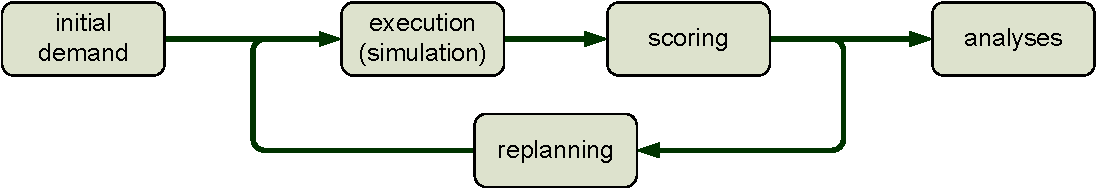
\includegraphics[width=1.0\textwidth, angle=90]{figures/MATSimLoop}}%
{Christoph Dobler}
%---------------------------------------------------------------------

\subsubsection{Multi-Figures}

Multi-Figures uses the same command as for single Figures. But instead
of adding one  ``\textbackslash{}includegraphics'' command in Item~\ref{item:singFig4}
you can add as many ``\textbackslash{}createsubfigure'' commands as you want.

The structure of the ``\textbackslash{}createsubfigure'' command is:
\begin{enumerate}
  \item\label{item:multFig1} the caption for the sub-figure
  \item\label{item:multFig2} the figure (again by using the
``\textbackslash{}includegraphics'' command)
  \item\label{item:multFig3} the label of the sub-figure
  \item\label{item:multFig4} either \textbackslash{}\textbackslash{} or leave it
empty
\end{enumerate}
The last item defines, if you want a line break between this
sub-figure and the following one. By using \textbackslash{}\textbackslash{} the
following figure will be on the next line. The last Sub-Figure should
not use \textbackslash{}\textbackslash{}.

\Cref{fig:labelOfTheMultiFigure1} contains two sub-figures
(\cref{fig:labelOfTheMultiFigure1-SubFig1,fig:labelOfTheMultiFigure1-SubFig2}) put on the same
line.

%---------------------------------------------------------------------
\createfigure%
{Multi-Figure1: Short Caption}%
{Multi-Figure1: Long Caption}%
{\label{fig:labelOfTheMultiFigure1}}%
{%
  \createsubfigure%
  {Caption of the first Sub-Figure}%
  {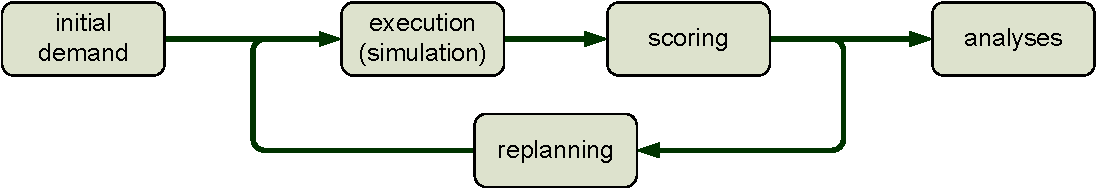
\includegraphics[width=0.49\textwidth,
angle=0]{figures/MATSimLoop}}%
  {\label{fig:labelOfTheMultiFigure1-SubFig1}}%
  {}%
  \createsubfigure%
  {Caption of the second Sub-Figure}%
  {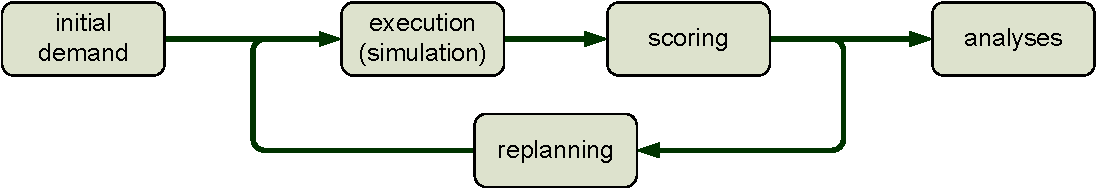
\includegraphics[width=0.49\textwidth,
angle=0]{figures/MATSimLoop}}%
  {\label{fig:labelOfTheMultiFigure1-SubFig2}}%
  {}%
}%
{}
%---------------------------------------------------------------------

\Cref{fig:labelOfTheMultiFigure2} contains three sub-figures
(\cref{fig:labelOfTheMultiFigure2-SubFig1,fig:labelOfTheMultiFigure2-SubFig2,fig:labelOfTheMultiFigure2-SubFig3}). The first one is set
on the first line, while the other two are set to the second line.

%---------------------------------------------------------------------
\createfigure%
{Multi-Figure2: Short Caption}%
{Multi-Figure2: Long Caption}%
{\label{fig:labelOfTheMultiFigure2}}%
{%
  \createsubfigure%
  {Caption of the first Sub-Figure}%
  {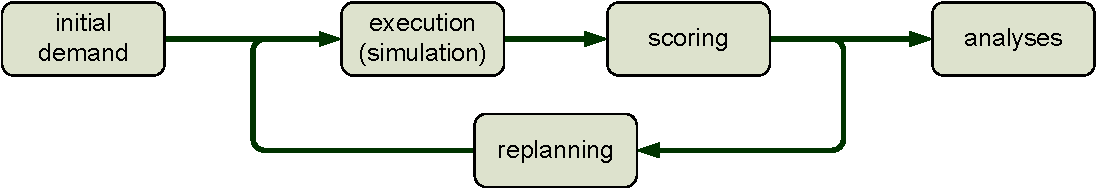
\includegraphics[width=0.70\textwidth,
angle=0]{figures/MATSimLoop}}%
  {\label{fig:labelOfTheMultiFigure2-SubFig1}}%
  {\\}%
  \createsubfigure%
  {Caption of the second Sub-Figure}%
  {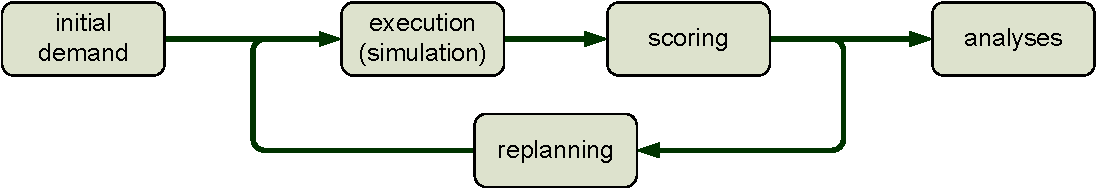
\includegraphics[width=0.48\textwidth,
angle=0]{figures/MATSimLoop}}%
  {\label{fig:labelOfTheMultiFigure2-SubFig2}}%
  {\hfill}%
  \createsubfigure%
  {Caption of the third Sub-Figure}%
  {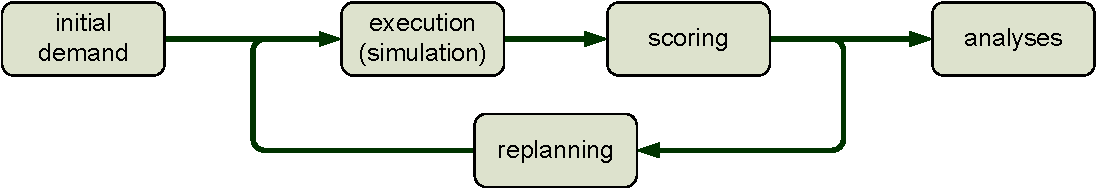
\includegraphics[width=0.48\textwidth,
angle=0]{figures/MATSimLoop}}%
  {\label{fig:labelOfTheMultiFigure2-SubFig3}}%
  {}%
}%
{my source}
%---------------------------------------------------------------------

\subsubsection{Landscape figures}

Oversize figures in landscape orientation can be put rotated
on a separate page
using the ``\textbackslash{}createsidewaysfigure''
command,
only that no placement specifier is available.
The syntax is identical to that of the
``\textbackslash{}createfigure''
command (cf.~\cref{sec:compStructs-Figures-SingleFigures}).
The page is rotated for on-screen display, too.
The result can be seen in \cref{fig:loop-page}.
\createsidewaysfigure{%
MATSim simulation loop}{%
The MATSim simulation loop}{%
% Used when referring to the figure
\label{fig:loop-page}%
}
{%
% Command that loads the figure.
% Supported formats: PDF, PNG and JPEG.
% File extension can be omitted
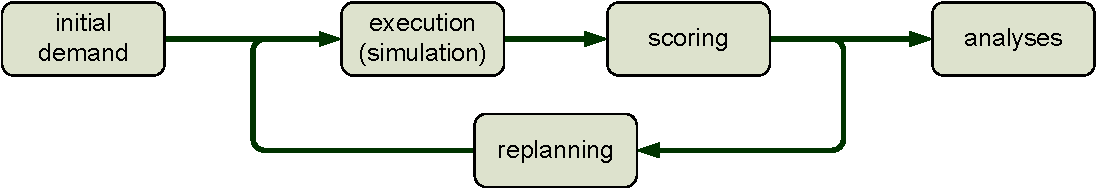
\includegraphics[width=\linewidth]{figures/MATSimLoop}%
}{%
% The source (now mandatory, but can be empty)
Christoph Dobler%
}


%%%%%%%%%%%%%%%%%%%%%%%%%%%%%%%%%%%%%%%%%%%%%%%%%%%%%%%%%%%%%%%%%%%%%%
\subsection{Tables} \label{sec:compStructs-Tables}
%%%%%%%%%%%%%%%%%%%%%%%%%%%%%%%%%%%%%%%%%%%%%%%%%%%%%%%%%%%%%%%%%%%%%%

A table has the same structure as the single Figure (see above). But
instead of including a graphic in item~4 you add the ``tabular''
construct. Unfortunately it is not that easy to understand and edit such a table. One has
to get used to it. However, quite a few tools can help converting the data
to the \LaTeX{} format, see \url{http://tex.stackexchange.com/q/49414/8057}
for an overview.

If you do not like it you can still add the table
as a graphic (with the ``\textbackslash{}includegraphics'') command.
But you still need to use the ``\textbackslash{}createtable'' command,
otherwise your table will appear
in the list of figures instead of the list of tables.
\Cref{tab:labelOfTheTable} shows an example of a table.

%---------------------------------------------------------------------
\createtable%
{A Tables short Caption}%
{A Tables long Caption}%
{\label{tab:labelOfTheTable}}%
{%
  \begin{tabular}[c]{lr@{.}lcr@{.}l}
    \toprule
    Bias / Error     & \multicolumn{2}{c}{Routes Only} &
\multicolumn{3}{c}{Times and Routes} \\
    \midrule
    Mean Abs. Bias:  & $+$331&40                        && $+$306&32  
                         \\
    Mean Rel. Bias:  &  $+$19&62\%                      &&  $+$25&27\%
                         \\
    \midrule
    Mean Abs. Error: &    533&55                        &&    503&77  
                         \\
    Mean Rel. Error: &     37&50\%                      &&     35&38\%
                         \\
    \bottomrule
  \end{tabular}
}%
{my source}
%---------------------------------------------------------------------

There is an analogous command ``\textbackslash{}createsubtable'' for multi-tables.

%%%%%%%%%%%%%%%%%%%%%%%%%%%%%%%%%%%%%%%%%%%%%%%%%%%%%%%%%%%%%%%%%%%%%%
\subsection{Pretty Printing}
%%%%%%%%%%%%%%%%%%%%%%%%%%%%%%%%%%%%%%%%%%%%%%%%%%%%%%%%%%%%%%%%%%%%%%

\LaTeX{} provides several functionalities for printing nice code, data
and so on. At the moment the layout features a nice way of printing
XML code. You do not have to copy XML into this paper, instead you can
include an XML file.
The command is similar to the Figure (it also will be included into
the list of figures). \Cref{fig:xml-plan} shows an example.

%---------------------------------------------------------------------
\createxmlfigure%
{A typical plan in XML.}%
{A typical plan in XML. This agent, id 393241, leaves home (on link
id 5834 of the given network) at 7:00~AM (performing home activity
for 7~hours), and drives to work via a four-node route (five links)
which it expects to take 25~minutes to traverse.  The agent stays at
work for 9~hours, then drives home again via a two-node route and
stays at home until midnight. Therefore, it describes a complete
day-plan for person number 393241.}%
{\label{fig:xml-plan}}%
{listings/examplePlans.xml}%
{}
%---------------------------------------------------------------------

If you want other pretty printing options, please ask
kirill.mueller@ivt.baug.ethz.ch.


%%%%%%%%%%%%%%%%%%%%%%%%%%%%%%%%%%%%%%%%%%%%%%%%%%%%%%%%%%%%%%%%%%%%%%
%
\section{Summary and Important Notes}
%
%%%%%%%%%%%%%%%%%%%%%%%%%%%%%%%%%%%%%%%%%%%%%%%%%%%%%%%%%%%%%%%%%%%%%%

This example paper gives you a short overview of how to write a paper
in \LaTeX{} inside the IVT \LaTeX{}-Bib\TeX{} environment. 
Some of the
concepts are general while other are made for the use at the IVT using
the IVT \LaTeX{} environment.

If you want to know more about \LaTeX, there is a pretty good and not
too long introduction under
\url{http://www.ctan.org/tex-archive/info/lshort/english/lshort.pdf}.
Even more can be found under \url{http://www.ctan.org/}. Also using
Google search engine helps a lot.

At last, there are some very important notes about writing in \LaTeX:
Since it is not a WYSIWYG way of writing papers, you always need to
``compile'' it to pdf. Unfortunately, if you do something wrong (i.e.\
forgetting a closing bracket, using non ISO characters, or using
special character that \TeX\ will interpret in another way) then error
messages will appear that are very very hard to understand. Therefore,
if you add something special, i.e.\ a figure, a table, a new Bib\TeX\
entry or a formula, compile the paper right before and right after you
added such stuff. If errors occurs, then you will at least know that
the produced error is caused by the last thing you did. That helps a
lot!

And something helps a lot, too: There are already many papers,
dissertations, CVs, misc stuff, etc., that you can find under
\texttt{ivt/doc}, that shows you very good examples what you can do
with \LaTeX.

If you have questions do not hesitate to ask someone at the IVT with a
bit of experience (Kirill, Basil, \ldots).



%%%%%%%%%%%%%%%%%%%%%%%%%%%%%%%%%%%%%%%%%%%%%%%%%%%%%%%%%%%%%%%%%%%%%%
%
\section*{\ackname}%
\addcontentsline{toc}{section}{\ackname}%
%
%%%%%%%%%%%%%%%%%%%%%%%%%%%%%%%%%%%%%%%%%%%%%%%%%%%%%%%%%%%%%%%%%%%%%%

State your acknowledgements here. 

%%%%%%%%%%%%%%%%%%%%%%%%%%%%%%%%%%%%%%%%%%%%%%%%%%%%%%%%%%%%%%%%%%%%%%
%% Bibliography
%%   Leave this as is, and add you own entries to my.bib
%%   Many references are already defined in _latexfiles/bibs/all-eng.bib
%%   Refer to the BibTeX/LaTeX tutorial for adding new entries
%%   to the IVT BibTeX database
%\bibliography{\mypath../_latexfiles/bibs/all-eng,my}
\bibliography{all-eng,my}
%%%%%%%%%%%%%%%%%%%%%%%%%%%%%%%%%%%%%%%%%%%%%%%%%%%%%%%%%%%%%%%%%%%%%%

%%%%%%%%%%%%%%%%%%%%%%%%%%%%%%%%%%%%%%%%%%%%%%%%%%%%%%%%%%%%%%%%%%%%%%
%% Appendices
%%   Usually they would start on a separate page
%%%%%%%%%%%%%%%%%%%%%%%%%%%%%%%%%%%%%%%%%%%%%%%%%%%%%%%%%%%%%%%%%%%%%%

\clearpage
\appendix

%%%%%%%%%%%%%%%%%%%%%%%%%%%%%%%%%%%%%%%%%%%%%%%%%%%%%%%%%%%%%%%%%%%%%%
%
\section{First section in the appendix} \label{sec:a1}
%
%%%%%%%%%%%%%%%%%%%%%%%%%%%%%%%%%%%%%%%%%%%%%%%%%%%%%%%%%%%%%%%%%%%%%%

The appendix starts with the ``appendix'' command. the rest is the same as in the sections.

%%%%%%%%%%%%%%%%%%%%%%%%%%%%%%%%%%%%%%%%%%%%%%%%%%%%%%%%%%%%%%%%%%%%%%
\subsection{A subsection in the appendix} \label{sec:a1-subsection}
%%%%%%%%%%%%%%%%%%%%%%%%%%%%%%%%%%%%%%%%%%%%%%%%%%%%%%%%%%%%%%%%%%%%%%

bla bla bla bla bla bla bla bla bla bla bla bla bla bla bla bla bla bla bla bla bla bla bla bla bla bla bla bla bla bla bla bla bla bla bla bla bla bla

bla bla bla bla bla bla bla bla bla bla bla bla
bla bla bla bla bla bla bla bla bla bla bla bla bla bla bla bla bla bla bla bla bla bla bla bla bla bla bla bla bla bla bla bla bla bla bla bla bla bla bla bla bla bla bla bla bla bla bla bla bla bla bla bla bla bla bla bla bla bla bla bla bla bla bla bla bla bla bla bla bla bla bla bla bla bla bla bla bla bla bla bla bla bla bla bla bla bla bla bla bla bla bla bla bla bla bla bla bla bla bla bla
bla bla bla bla bla bla bla bla bla bla bla bla bla bla bla bla bla bla bla bla bla bla bla bla bla bla bla bla bla bla bla bla bla bla bla bla bla bla bla bla

%%%%%%%%%%%%%%%%%%%%%%%%%%%%%%%%%%%%%%%%%%%%%%%%%%%%%%%%%%%%
\section{Second section in the appendix}
%%%%%%%%%%%%%%%%%%%%%%%%%%%%%%%%%%%%%%%%%%%%%%%%%%%%%%%%%%%%

bla bla bla bla bla bla bla bla bla bla bla bla
bla bla bla bla bla bla bla bla bla bla bla bla bla bla bla bla bla bla bla bla bla bla bla bla bla bla bla bla bla bla bla bla bla bla bla bla bla bla bla bla bla bla bla bla bla bla bla bla bla bla bla bla bla bla bla bla bla bla bla bla bla bla bla bla bla bla bla bla bla bla bla bla bla bla bla bla bla bla bla bla bla bla bla bla bla bla bla bla bla bla bla bla bla bla bla bla bla bla bla bla
bla bla bla bla bla bla bla bla bla bla bla bla bla bla bla bla bla bla bla bla bla bla bla bla bla bla bla bla bla bla bla bla bla bla bla bla bla bla bla bla


\end{document}

%%%%%%%%%%%%%%%%%%%%%%%%%%%%%%%%%%%%%%%%%%%%%%%%%%%%%%%%%%%%%%%%%%%%%%
%%%%%%%%%%%%%%%%%%%%%%%%%%%%%%%%%%%%%%%%%%%%%%%%%%%%%%%%%%%%%%%%%%%%%%
%%
%% END OF DOCUMENT
%%
%%%%%%%%%%%%%%%%%%%%%%%%%%%%%%%%%%%%%%%%%%%%%%%%%%%%%%%%%%%%%%%%%%%%%%
%%%%%%%%%%%%%%%%%%%%%%%%%%%%%%%%%%%%%%%%%%%%%%%%%%%%%%%%%%%%%%%%%%%%%%

%%%%%%%%%%%%%%%%%%%%%%%%%%%%%%%%%%%%%%%%%%%%%%%%%%%%%%%%%%%%%%%%%%%%%%
%% Editor specific keywords:
%%   This is not part of you paper, but sometimes it is used
%%   for additional features of TeX Editors.
%%
%% WinEdt:
%%   to get the bibliography list
%GATHER{./_bibs/all-eng.bib}
